\chapter{Nuevo Sistema de Entrenamiento}\label{chap:2}
En este capítulo se presentará la propuesta de solución para este nuevo sistema de entrenamiento que se desea conseguir. Para que el desarrollo de un proyecto concluya con éxitos, primero debe realizarse un diseño completo de lo que se pretende obtener, así como los recursos y requisitos que debe poseer. A lo largo del capítulo se tratarán de presentar numerosos diagramas para facilitar la comprensión. Cabe destacar que este nuevo diseño parte del SECPROIT, por lo que se realizarán algunas comparaciones con ese sistema.

\section{Modelado del Negocio}
Los modelos se crean con el objetivo de entender mejor la entidad real que se va a construir. Deben cumplir con objetivos diferentes, niveles de abstracción, con la ilustración del software desde el punto de vista del cliente y después con su representación en un nivel más técnico.

\subsection{Modelo de Dominio}
El modelo de dominio es una representación de las clases conceptuales del mundo real, no de componentes de software. Se muestran los conceptos significativos en un dominio del problema. Para una mejor comprensión del modelo, es necesario entender las entidades que influyen en el negocio.

En la Figura \ref{fig:modelD}, se puede apreciar el modelo de dominio para este nuevo sistema. Es muy semejante, en cuanto a lógica del negocio, al modelo del SECPROT.

Las áreas de color verde, indica que se ha modificado la entidad para ajustarla a los nuevos cambios que se decidieron hacer. Los cambios más significativos son aquellas entidades que se modificaron casi en su totalidad o aquellas que fueron agregadas de cero. Estas últimas están representadas con un color amarillo. 

\begin{figure}[h]
\centering
 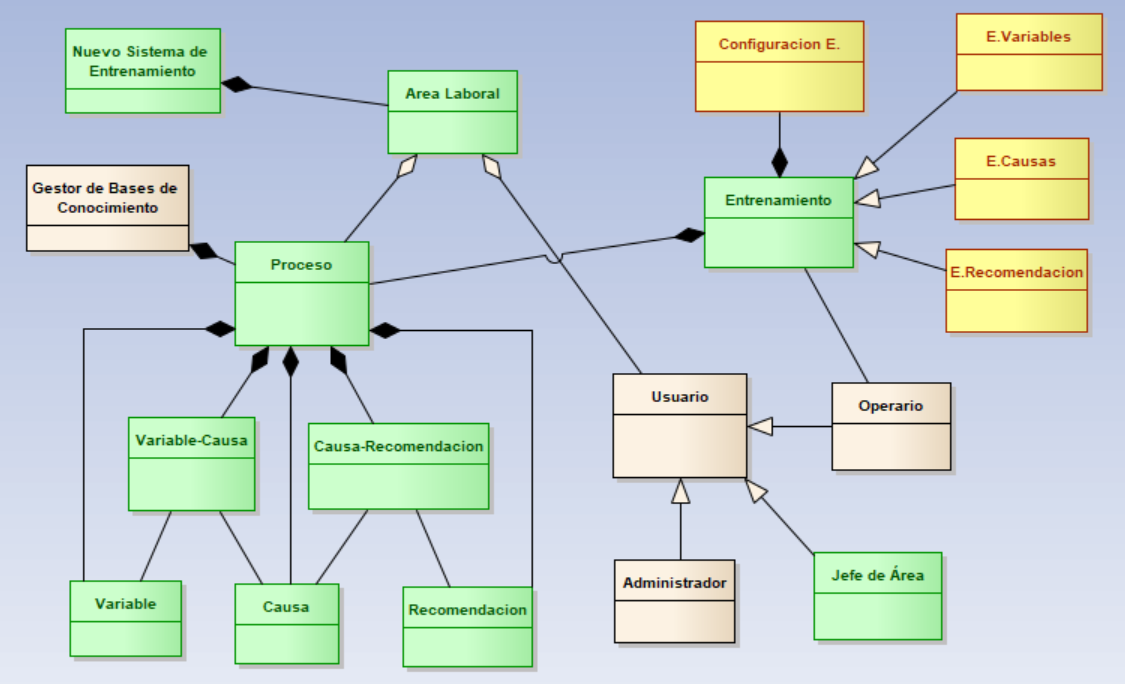
\includegraphics[width=0.8\linewidth]{imagen/dominio.png}
 \caption{Modelo de Dominio del Nuevo Sistema.}
 \label{fig:modelD} 
\end{figure} 

Como bien se aprecia, el diagrama indica que se han creado cuatro nuevas entidades: configuración de entrenamiento, entrenamiento de variables, entrenamiento de causas y entrenamiento de recomendaciones. Estas entidades fueron creadas para un mejor manejo de la información de la capacitación, y para introducir una nueva regla: separar los entrenamientos por etapas.

\subsection{Reglas del Negocio}
Cada negocio posee un conjunto de restricciones que permiten su correcto funcionamiento. Estas restricciones son conocidas como reglas del negocio.
Las reglas a cumplir en este nuevo sistemas son:

\begin{itemize}
\item Antes de crear un usuario, deben haberse creado los roles del sistema y las áreas laborales.
\item Antes de crear un proceso, deben haberse creado las áreas laborales.
\item Antes de crear un entrenamiento debe existir un proceso y al menos un operario.
\item Antes de realizar el entrenamiento de las causas se debe haber aprobado el entrenamiento de las variables.
\item Antes de realizar el entrenamiento de las recomendaciones se debe haber aprobado el entrenamiento de las causas.
\item Los usuarios solo pueden poseer un rol.
\item Los usuarios solo pueden pertenecer a un área a la vez.
\item Los procesos solo pueden pertenecer a un área a la vez.
\item Las tareas de los roles son únicas para el usuario, es decir, solo las pueden hacer los usuarios con el mismo rol.
\end{itemize} 

\subsection{Diagrama de Actividades}
Un diagrama de actividades recoge una vista dinámica de alto nivel, del flujo principal del proceso. En el mismo, se tienen en cuenta las entidades que participan en el negocio y las acciones que realizan cada una, así como los llamados objetos con los que se trabaja. En estos diagramas se representa el inicio y el fin del flujo.

En esta propuesta de solución, el flujo del administrador resulta el mismo que el del sistema SECPROIT \cite{elena}. Sin embargo, el flujo de los operarios y jefes de área cambia. En la Figura \ref{fig:actividades}, se representa el diagrama de actividades de estos dos roles, detallando el nuevo flujo de los mismos.

\begin{figure}[h]
\centering
 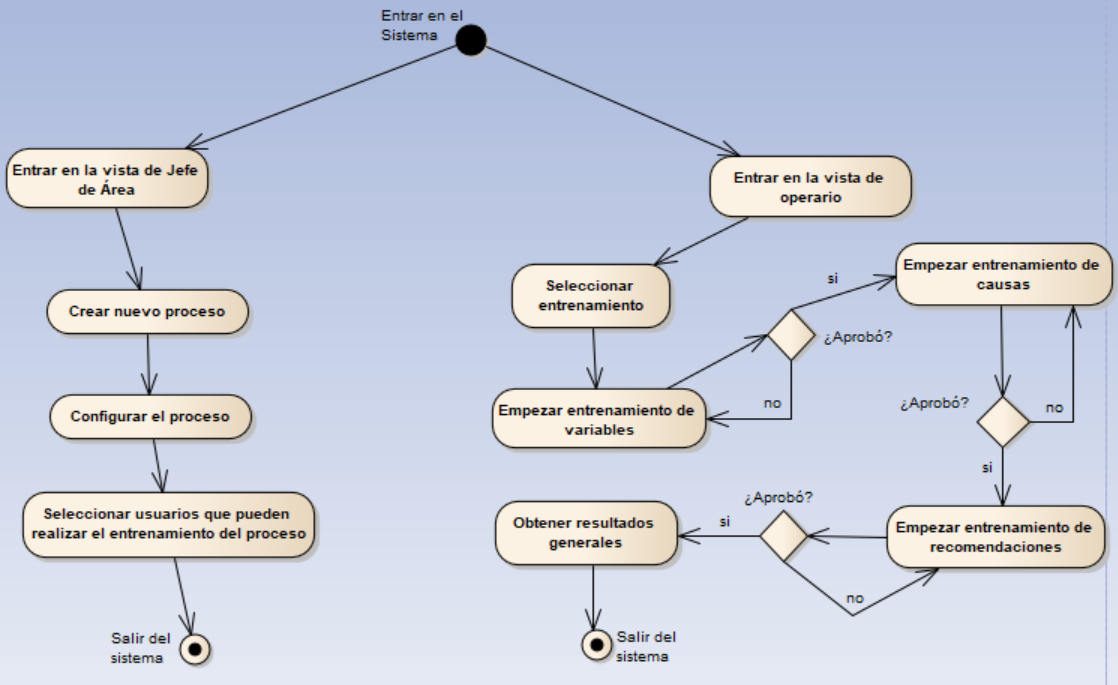
\includegraphics[width=0.8\linewidth]{imagen/actividades.png}
 \caption{Diagrama de Actividades del Nuevo Sistema.}
 \label{fig:actividades} 
\end{figure} 

%%%%%%%%%%%%%%%%%%%%%%%%%%%%%%%%

\section{Captura de Requisitos}
En la captura de requisitos se obtiene el modelo del sistema a desarrollar, quedando definidas las funcionalidades requeridas para establecer las fronteras del sistema. Además, se proponen otros elementos para lograr un mayor grado de especificación en el propio modelado del sistema.

\subsection{Requisitos Funcionales}
Los requisitos funcionales denotan las funcionalidades del sistema. Estos son 
capacidades o condiciones que se deben cumplir. Las funcionalidades del nuevo sistema son:

\begin{itemize}
\item \textsl{Gestionar Usuarios:} es una actividad desarrollada por los administradores. Se basa en introducir, modificar y desactivar usuarios en el sistema. También cuentan con una opción para restablecer la contraseña de los usuarios, en caso de que estos las hayan olvidado.
\item \textsl{Gestionar Áreas:}  es una actividad desarrollada por los administradores. Se basa en introducir, modificar y eliminar las áreas del sistema. Para poder eliminar un área laboral, esta debe estar vacía, es decir, que de ella no dependan ni procesos ni usuarios.
\item \textsl{Ver Acciones de los Usuarios:}  es una actividad desarrollada por los administradores, que les permite ver todas las actividades relacionadas con el sistema, realizadas por los usuarios. A modo de resumen, registra los camios realizados junto al nombre del usuario que lo hizo.
\item \textsl{Cambiar Contraseña:} es una acción que todos los usuarios pueden realizar.
\item \textsl{Entrar en el Sistema:} es una acción que todos los usuarios pueden realizar. Consiste en introducir las credenciales (nombre de usuario y contraseña) en el sistema.
\item \textsl{Gestionar Procesos:} es una actividad desarrollada por los jefes de área. Se basa en introducir, modificar y eliminar los procesos en un área laboral. Si se elimina un proceso, queda registro del mismo y los entrenamientos que se hayan realizado no se pierden.
\item \textsl{Configurar Entrenamiento:}  es una actividad desarrollada por los jefes de área. Consiste en asignar para cada proceso, la cantidad de pruebas por etapas, los estilos de pregunta que se pueden aplicar, la cantidad general de intentos que se pueden realizar y los usuarios que pueden entrenar este proceso.
\item \textsl{Realizar Entrenamiento:} es una acción desarrollada por los operarios. Consiste en responder las preguntas de los entrenamientos.
\end{itemize}

\subsection{Requisitos No Funcionales}
Los requisitos no funcionales son propiedades, características y restricciones que se deben presentar el sistema, asegurando el cumplimiento de las acciones demandadas. Los requisitos no funcionales de esta propuesta de solución son:

\begin{itemize}
\item \textsl{Usabilidad:} se debe garantizar un ambiente de trabajo simple e intuitivo, ya que la mayoría de los usuarios no poseen experiencias con sistemas informáticos.
\item \textsl{Seguridad:} la información del sistema solo puede ser manipulada por usuarios autorizados (aquellos que posean usuario y contraseña). Las actividades deben estar divididas por roles, lo que presenta menor riesgo de errores.
\item \textsl{Confiabilidad:} se debe evitar los enlaces rotos. La información contenida en los ficheros de los procesos, se debe validar antes de ser usada, para evitar errores. Se debe garantizar la confidencialidad de la información.
\item \textsl{Disponibilidad:} la aplicación de mecanismos de seguridad no debe constituir un retraso para el uso del sistema. El software siempre debe estar disponible, así como brindar su información actualizada.
\item \textsl{Software:} se debe tener instalado el JDK versión 1.8 y la aplicación PostgreSQL versión 9.1 (como mínimo). Esta última se utiliza como gestor de base de datos.
\item \textsl{Hardware:} se necesitan 64MB de memoria RAM, un microprocesador Pentium II a 450 MHz como mínimo, y un disco duro con capacidad libre mínima de 4 GB, para almacenar la nueva información incorporada. Además, es necesario un sistema operativo de entorno gráfico como Windows y Linux y que estén establecidas las condiciones necesarias para el acceso al servidor.
\item \textsl{Portabilidad:} debe ser utilizado bajo sistemas operativos Windows o Linux, por lo que su desarrollo debe realizarse con un lenguaje y tecnologías capaces de brindar este soporte. Además, el hecho de ser multiplataforma permite que el sistema llegue a un mayor número de personas. 
\item \textsl{Restricciones en el diseño y la implementación:} debe desarrollarse sobre plataformas de software libre y código abierto. Además, se utiliza la herramienta \textsl{Drools}, por lo tanto, el lenguaje de programación debe ser Java.
\item \textsl{Políticos/Culturales:} debe encontrarse en idioma español.
\end{itemize}

%%%%%%%%%%%%%%%%%%%%%%%%%%%%%%%%

\section{Casos de Uso del Nuevo Sistema}
Los casos de uso del sistema establecen un acuerdo entre clientes y desarrolladores sobre las condiciones y requisitos que debe cumplir la aplicación. Es un artefacto narrativo que describe, bajo la forma de acciones y reacciones, el comportamiento del sistema desde el punto de vista del usuario.

\subsection{Actores del Sistema} 
Un actor del sistema es una entidad externa relacionada con el mismo y que demanda una funcionalidad. Esto incluye a los operadores humanos, pero también incluye a todos los sistemas externos. En la Tabla \ref{tab:actores}, se muestran todos los actores del nuevo sistema y una breve explicación de los mismos:

\begin{table}[h]
\begin{center}
\begin{tabular}{ | c | p{7.8cm} | }
\hline
\textbf{Actor} & \textbf{Descripción} \\
\hline
Usuario & Es el actor genérico que hace uso de las funcionalidades que son comunes. \\
\hline
Operario & Es el actor que se evalúa a partir de los entrenamientos de los procesos. \\
\hline
Jefe de Área & Es el actor que vincula los procesos en las áreas y los configura, decidiendo qué usuarios se entrenarán y las características que deberán cumplir para aprobar. Anteriormente era conocido como Especialista. \\
\hline
Administrador & Es el actor que gestiona las áreas, los usuarios y visualiza las operaciones realizadas por los mismos. \\
\hline
Generador de Bases de Conocimientos & Es un sistema externo que genera las bases de conocimientos con las que se trabaja en los entrenamientos (procesos). \\
\hline
\end{tabular}
\caption{Actores del Nuevo Sistema.}
\label{tab:actores}
\end{center}
\end{table}

\subsection{Diagrama de Casos de Uso del Nuevo Sistema}
Un caso de uso es una secuencia de interacciones entre un sistema y alguien o algo que usa alguno de sus servicios. Describen tanto lo que hace el actor como la repuesta que recibe, aunque el énfasis está puesto en la interacción. Es iniciado por un actor y, a partir de ese momento, se intercambian datos. En la Figura \ref{fig:casoUso}, se puede observar el diagrama de casos de uso del nuevo sistema.

El diagrama, en general, tiene como base el sistema SECPROIT, pero con algunas modificaciones incluidas. Los casos de uso que se encuentran de color verde, indican que, en principio, realizan las mismas operaciones, pero con cambios incorporados. El actor del mismo color se debe a que cambió de nombre, de especialista a jefe de área. El caso de uso de color amarillo, es completamente nuevo.

\begin{figure}[h]
\centering
 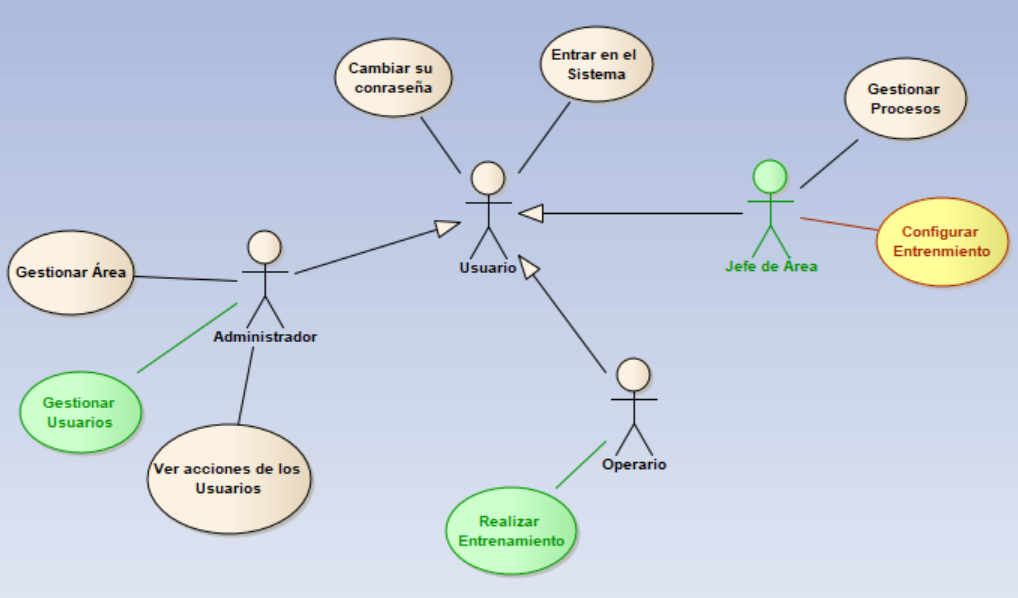
\includegraphics[width=0.8\linewidth]{imagen/casoUso.png}
 \caption{Diagrama de Casos de Uso del Nuevo Sistema.}
 \label{fig:casoUso} 
\end{figure}

%%%%%%%%%%%%%%%%%%%%%%%%%%%%%%%%

\section{Modelo de Datos}
En el desarrollo de esta herramienta se utiliza: una bases de datos en PostgreSQL y un grupo de ficheros \textsl{anm} y \textsl{drl} que conforman los proceso de los entrenamientos. En la base de datos se almacena toda la información referente al sistema: los datos de los usuarios, los resultados de los entrenamientos, los procesos, la información de las áreas y una lista detallada de todas las operaciones realizadas en el sistema.

\subsection{Diagrama de Entidades y Relaciones (DER)}
Un Diagrama de Entidades y Relaciones (DER) representa las clases del sistema, con sus atributos, y las relaciones existentes entre ellas.